%15 min preso!
\documentclass[xcolor=table,aspectratio=169]{beamer}
\usepackage{beamerthemesplit}
\usepackage{wrapfig}
\usetheme{SPbGU}
\usepackage{pdfpages}
\usepackage{amsmath}
\usepackage{cmap}
\usepackage[T2A]{fontenc}
\usepackage[utf8]{inputenc}
\usepackage[english]{babel}
\usepackage{indentfirst}
\usepackage{amsmath}
\usepackage{tikz}
\usepackage{multirow}
\usepackage[noend]{algpseudocode}
\usepackage{algorithm}
\usepackage{algorithmicx}
\usepackage{fancyvrb}
\usepackage{hyperref} 
\definecolor{links}{HTML}{2A1B81}
\hypersetup{colorlinks,linkcolor=,urlcolor=links}
\usetikzlibrary{calc}
\usetikzlibrary{shapes, backgrounds}
\usetikzlibrary{arrows,automata}
\usetikzlibrary{positioning}
\usetikzlibrary{fit}
\usetikzlibrary{shapes.callouts}
\usetikzlibrary{shapes.misc}
\usepackage{xparse}
\usepackage{fontawesome}

\usepackage{etoolbox,refcount}
\usepackage{multicol}

\usepackage{tabularx}
\newcolumntype{Y}{>{\raggedleft\arraybackslash}X}

\renewcommand{\thealgorithm}{}

\newtheorem{mytheorem}{Theorem}
\renewcommand{\thealgorithm}{}

\newcommand{\tikzmark}[1]{\tikz[overlay,remember picture] \node (#1) {};}
\def\Put(#1,#2)#3{\leavevmode\makebox(0,0){\put(#1,#2){#3}}}

\newcommand{\ltz}{$< 1$}

\tikzset{
    state/.style={
           rectangle,
           rounded corners,
           draw=black, very thick,
           minimum height=2em,
           inner sep=2pt,
           text centered,
           },
}

\tikzset{
    invisible/.style={opacity=0,text opacity=0},
    visible on/.style={alt=#1{}{invisible}},
    alt/.code args={<#1>#2#3}{%
      \alt<#1>{\pgfkeysalso{#2}}{\pgfkeysalso{#3}} % \pgfkeysalso doesn't change the path
    },
}

\tikzset{cross/.style={cross out, draw=black, minimum size=2*(#1-\pgflinewidth), inner sep=0pt, outer sep=0pt, ultra thick},
%default radius will be 1pt. 
cross/.default={1pt}}

\NewDocumentCommand{\mycallout}{r<> O{opacity=0.8,text opacity=1} m m m}{%
\tikz[remember picture, overlay]\node[align=center, fill=cyan!20, text width=#5cm,
#2,visible on=<#1>, rounded corners,
draw,rectangle callout,anchor=pointer,callout relative pointer={(290:0.5cm)}]
at (#3) {#4};
}

\NewDocumentCommand{\mycalloutR}{r<> O{opacity=0.8,text opacity=1} m m m}{%
\tikz[remember picture, overlay]\node[align=center, fill=cyan!20, text width=#5cm,
#2,visible on=<#1>, rounded corners,
draw,rectangle callout,anchor=pointer,callout relative pointer={(30:0.8cm)}]
at (#3) {#4};
}

\newcommand\colR{\cellcolor{red!20}}
\newcommand\colB{\cellcolor{blue!20}}
\newcommand\colG{\cellcolor{green!20}}
\definecolor{Gray}{gray}{0.8}

%callout relative pointer={(230:0.5cm)}]

\newcounter{countitems}
\newcounter{nextitemizecount}
\newcommand{\setupcountitems}{%
  \stepcounter{nextitemizecount}%
  \setcounter{countitems}{0}%
  \preto\item{\stepcounter{countitems}}%
}
\makeatletter
\newcommand{\computecountitems}{%
  \edef\@currentlabel{\number\c@countitems}%
  \label{countitems@\number\numexpr\value{nextitemizecount}-1\relax}%
}
\newcommand{\nextitemizecount}{%
  \getrefnumber{countitems@\number\c@nextitemizecount}%
}
\newcommand{\previtemizecount}{%
  \getrefnumber{countitems@\number\numexpr\value{nextitemizecount}-1\relax}%
}
\makeatother    
\newenvironment{AutoMultiColItemize}{%
\ifnumcomp{\nextitemizecount}{>}{3}{\begin{multicols}{2}}{}%
\setupcountitems\begin{itemize}}%
{\end{itemize}%
\unskip\computecountitems\ifnumcomp{\previtemizecount}{>}{3}{\end{multicols}}{}}


\beamertemplatenavigationsymbolsempty

\title[GraphBLAS+RISC-V+GPGPU]{Анализ графов и разреженная линейная алгебра GPGPU в экосистеме RISC-V}
\subtitle{Рабочая группа ``Развитие экосистемы ПО на RISC-V''}
\institute[СПбГУ]{
Санкт-Петербургский Государственный Университет
}

% То, что в квадратных скобках, отображается в левом нижнем углу.
\author[Семён Григорьев]{Семён Григорьев}

\date{29 августа 2025}

\begin{document}
{
\begin{frame}[fragile]
  \begin{table}
  \centering
  %
\includegraphics[height=1.5cm]{pictures/SPbGU_Logo.png}
  \begin{tabularx}{\linewidth}{XcX}
    %
\includegraphics[height=0.9cm]{pictures/hu_logo.jpeg} 
    \hfill
    & 
    & \hfill 
\includegraphics[height=1.6cm]{pictures/SPbGU_Logo.png}
  \end{tabularx}
  \end{table}
  \titlepage
\end{frame}
}


%\begin{frame}[fragile]
%  \frametitle{План доклада}
%  \begin{itemize}
%    \item RISC-V и GPGPU
%    \item Обработка графов и GPGPU
%    \item GraphBLAS и GPGPU
%    \item Направления работ, выводы 
%  \end{itemize}
%\end{frame}

\begin{frame}[fragile]
  \frametitle{RISC-V и GPGPU}
  \begin{itemize}
    \item \textbf{RISC-V CPU + Imagination Technologies GPU}: самая распространённая (из доступных) конфигурация
    \item \textbf{RISC-V CPU + AMD GPU}: утверждается, что работает и есть официальная поддержка (\href{https://milkv.io/pioneer}{Milk-V Pioneer}, \href{https://riscv.org/ecosystem-news/2024/10/risc-v-cpu-demoed-with-rx-7900-xtx-gpu-in-debian-linux-amd-flagship-gpu-paired-with-milk-v-megrez-board-and-sifive-p550-cores/}{Milk-V Megrez}, \href{https://milkv.io/ruyibook}{RuyiBook})
    \item \textbf{RISC-V CPU + Intel GPU}: \href{https://www.reddit.com/r/RISCV/comments/1ftep9u/intel_arc_a770_on_riscv/}{ходят слухи, что можно}, но официальной поддержки пока нет
    \item \textbf{RISC-V CPU + Nvidia GPU}: \href{https://riscv.org/ecosystem-news/2025/07/nvidia-to-bring-cuda-platform-support-to-the-risc-v/}{анонсировано}
    \item \textbf{RISC-V GPU}: \href{https://github.com/vortexgpgpu/vortex}{Vortex}
  \end{itemize}
  %\begin{center}        
  %  \begin{tabular}{c|c}
  %    Хост & GPGPU \\
  %    \hline
  %    \hline
  %    RISC-V &      
  %      OpenCL
  %      Nvidia Cuda \\
  %    \hline
  %   ? & RISC-V \\
  %  \end{tabular}
  %\end{center}
\end{frame}

\begin{frame}[fragile]
  \frametitle{Обработка графов на GPGPU}
  Нетривиальная задача из-за нерегулярного параллелизма
  \begin{itemize}
    \item \href{https://developer.nvidia.com/nvgraph}{NVGraph}
    \item \href{https://github.com/gunrock/gunrock}{Gunrock}    
    \item Различные системы, которые что-то умеют отдавать на ГПУ
    \item Частые решения отдельных задач
  \end{itemize}

\end{frame}


\begin{frame}[fragile]
  \frametitle{GraphBLAS и GPGPU}
  \begin{itemize}
    \item SuiteSparse:GraphBLAS
    \begin{itemize}
      \item Cuda
      \item Пока не анонсировано
    \end{itemize}
    \item GraphBLAST
    \begin{itemize}
      \item Cuda
      \item Очень небольшое подмножество
    \end{itemize}
    \item Spla
    \begin{itemize}
      \item OpenCL
      \item В разработке
    \end{itemize}
    \end{itemize}
\end{frame}

\begin{frame}[fragile]
  \frametitle{Spla\footnote{\url{https://github.com/SparseLinearAlgebra/spla}}}
  Реализация подмножества GraphBLAS-подобного API на C++ и OpenCL C
  \begin{itemize}
    \item Переносимое решение между GPGPU разных вендоров
    \item Запускается на CPU благодаря POCL
    \item На <<взрослых>> GPGPU конкурентно с аналогами    
  \end{itemize}
\end{frame}


\begin{frame}[t]
  \frametitle{Экспериментальное исследование}
  \begin{itemize}
    \item SuiteSparse matrix collection: матрицы разных размеров и разной степени разреженности
    \item Оборудование
    \begin{itemize}
    %\item X86\_64
    %\begin{itemize}
    %  \item \textbf{CPU}: Intel Core i7-12700H 800MHz с векторами размером 1024 битов
    %  \item \textbf{RAM}: LPDDR4, 16GB
    %  \item \textbf{Compiler}: GCC 14.2.0
    %\end{itemize}
    \item RISC-V
    \begin{itemize}
      \item \textbf{SoC}: SPACEMIT K1/M1, Octa-core X60™(RV64GCVB), RVA22, RVV1.0 1600MHz с векторами размером 2048 битов 
      \item \textbf{RAM}: LPDDR4X, 16GB 
     % \item \textbf{Compiler}: GCC 14.2.0 (cross)
    \end{itemize}
    \end{itemize}
    \item Замеряется время решения прикладной задачи (работы алгоритма)
    \item Подгрузка и конвертация данных не замеряется
    \item Ускорение относительно LaGraph
  \end{itemize}  
\end{frame}

\begin{frame}[t]
  \frametitle{Графы для экспериментов\footnote{Взяты типичные из SuiteSparse Matrix Collection}}
  \begin{center}
%    \resizebox{0.9\textwidth}{!}{
    \begin{table}[]
      \begin{tabular}{l|l|l|l|l|l}
      Name              & Vertices & Edges  & Avg Deg & Sd Deg & Max Deg  \\
      \hline\hline
      \rowcolor{Gray}
      coAuthorsCiteseer & 227.3K   & 1.6M   & 7.2     & 10.6   & 1372.0   \\
      coPapersDBLP      & 540.5K   & 30.5M  & 56.4    & 66.2   & 3299.0   \\
      \rowcolor{Gray}
      amazon-2008       & 735.3K   & 7.0M   & 9.6     & 7.6    & 1077.0   \\
      hollywood-2009    & 1.1M     & 112.8M & 98.9    & 271.9  & 11467.0  \\
      \rowcolor{Gray}
      belgium\_osm      & 1.4M     & 3.1M   & 2.2     & 0.5    & 10.0     \\
      roadNet-CA        & 2.0M     & 5.5M   & 2.8     & 1.0    & 12.0     \\
      \rowcolor{Gray}
      com-Orkut         & 3.1M     & 234.4M & 76.3    & 154.8  & 33313.0  \\
      cit-Patents       & 3.8M     & 33.0M  & 8.8     & 10.5   & 793.0    \\
      \rowcolor{Gray}
      rgg\_n\_2\_22\_s0 & 4.2M     & 60.7M  & 14.5    & 3.8    & 36.0     \\
      soc-LiveJournal   & 4.8M     & 85.7M  & 17.7    & 52.0   & 20333.0  \\
      \rowcolor{Gray}
      indochina-2004    & 7.4M     & 302.0M & 40.7    & 329.6  & 256425.0 \\
      rgg\_n\_2\_23\_s0 & 8.4M     & 127.0M & 15.1    & 3.9    & 40.0     \\
      \rowcolor{Gray}
      road\_central     & 14.1M    & 33.9M  & 2.4     & 0.9    & 8.0     
      \end{tabular}
    \end{table}
%}
  \end{center}
\end{frame}

\begin{frame}
  \frametitle{Результаты на SpacemiT M1 CPU, IMG BXE-2-32 GPU}

\begin{columns}
        \column{0.5\textwidth}        
        \vspace{-0.5cm}
        \begin{center}
          BFS \\
        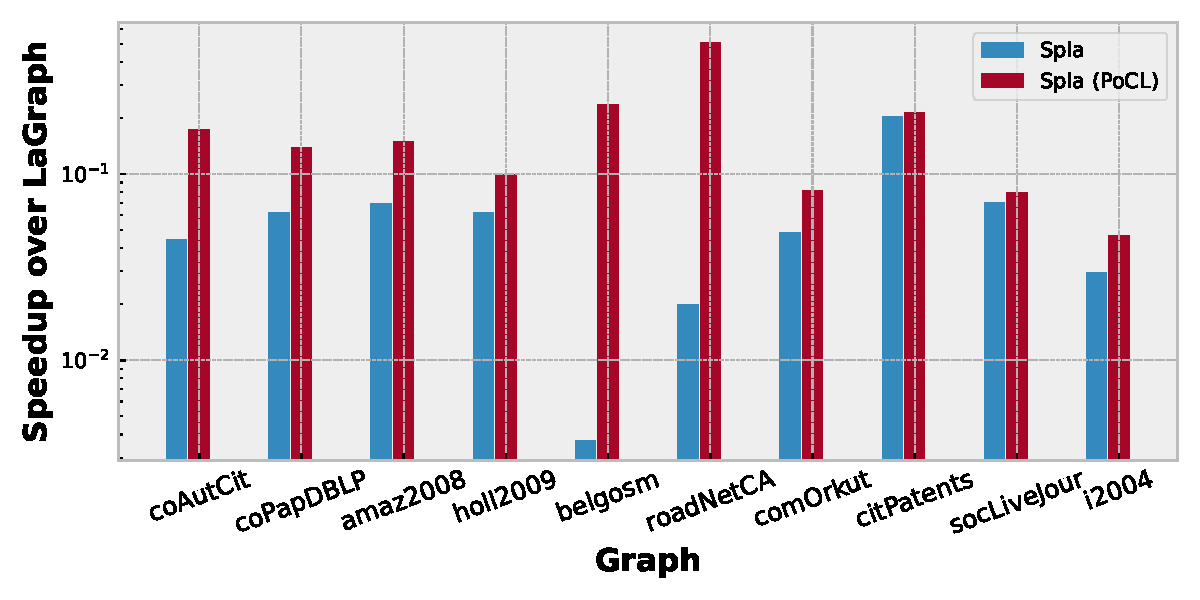
\includegraphics[width=0.909\linewidth]{pictures/rq1_rel_bfs.pdf}
        Single Source Shortest Path (SSSP) \\
        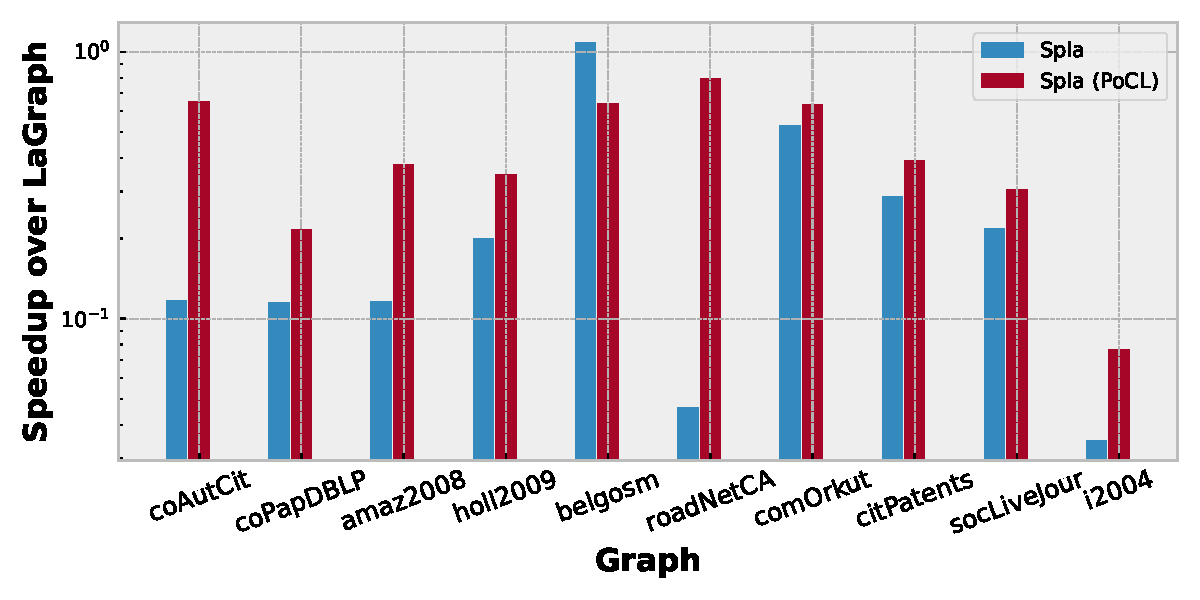
\includegraphics[width=0.909\linewidth]{pictures/rq1_rel_sssp.pdf}
        \end{center}
        \column{0.5\textwidth}
        \vspace{-0.5cm}
        \begin{center}
          Triangle Count (TC) \\
        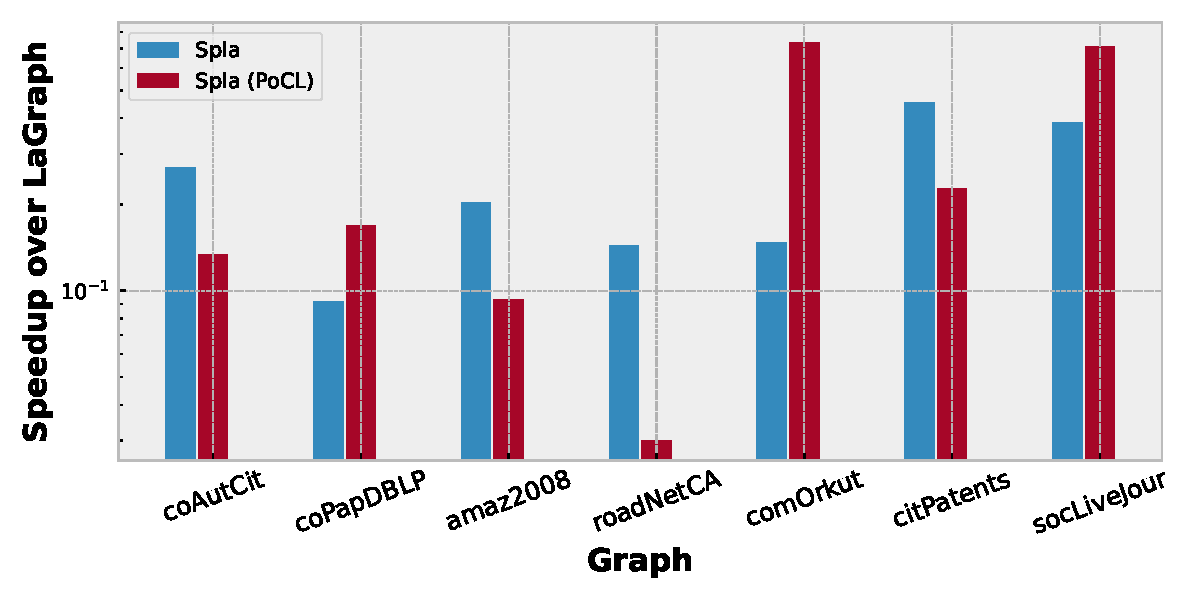
\includegraphics[width=0.9\linewidth]{pictures/rq1_rel_tc.pdf}
        PageRank (PR) \\
        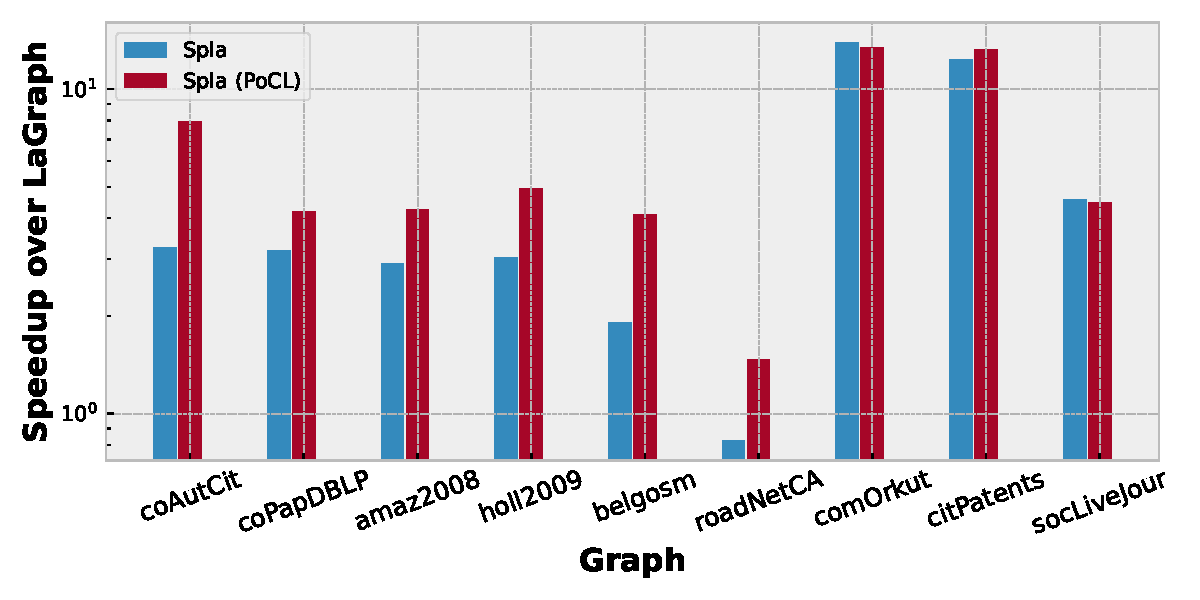
\includegraphics[width=0.9\linewidth]{pictures/rq1_rel_pr.pdf}
        \end{center}
    \end{columns}
    
\end{frame}

\begin{frame}
  \frametitle{Результаты на Nvidia GTX 1070}
  \begin{center}
    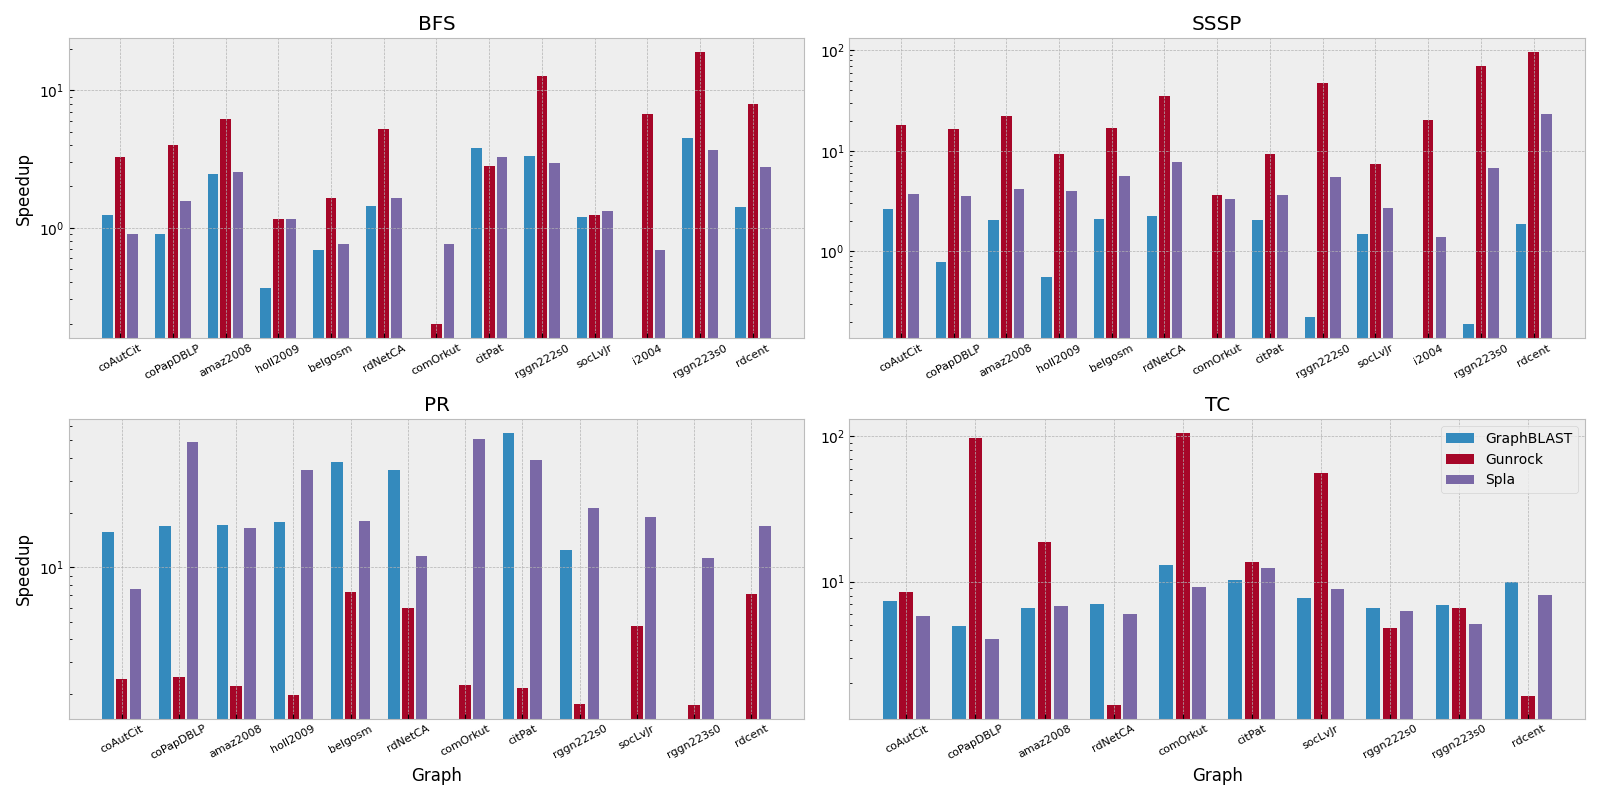
\includegraphics[width=0.85\linewidth]{pictures/rq1_rel.png}
    \\
    GPGPU не всегда полезен
  \end{center}
\end{frame}

\begin{frame}
  \frametitle{Результаты ГПН от Intel и AMD}
  \begin{center}
    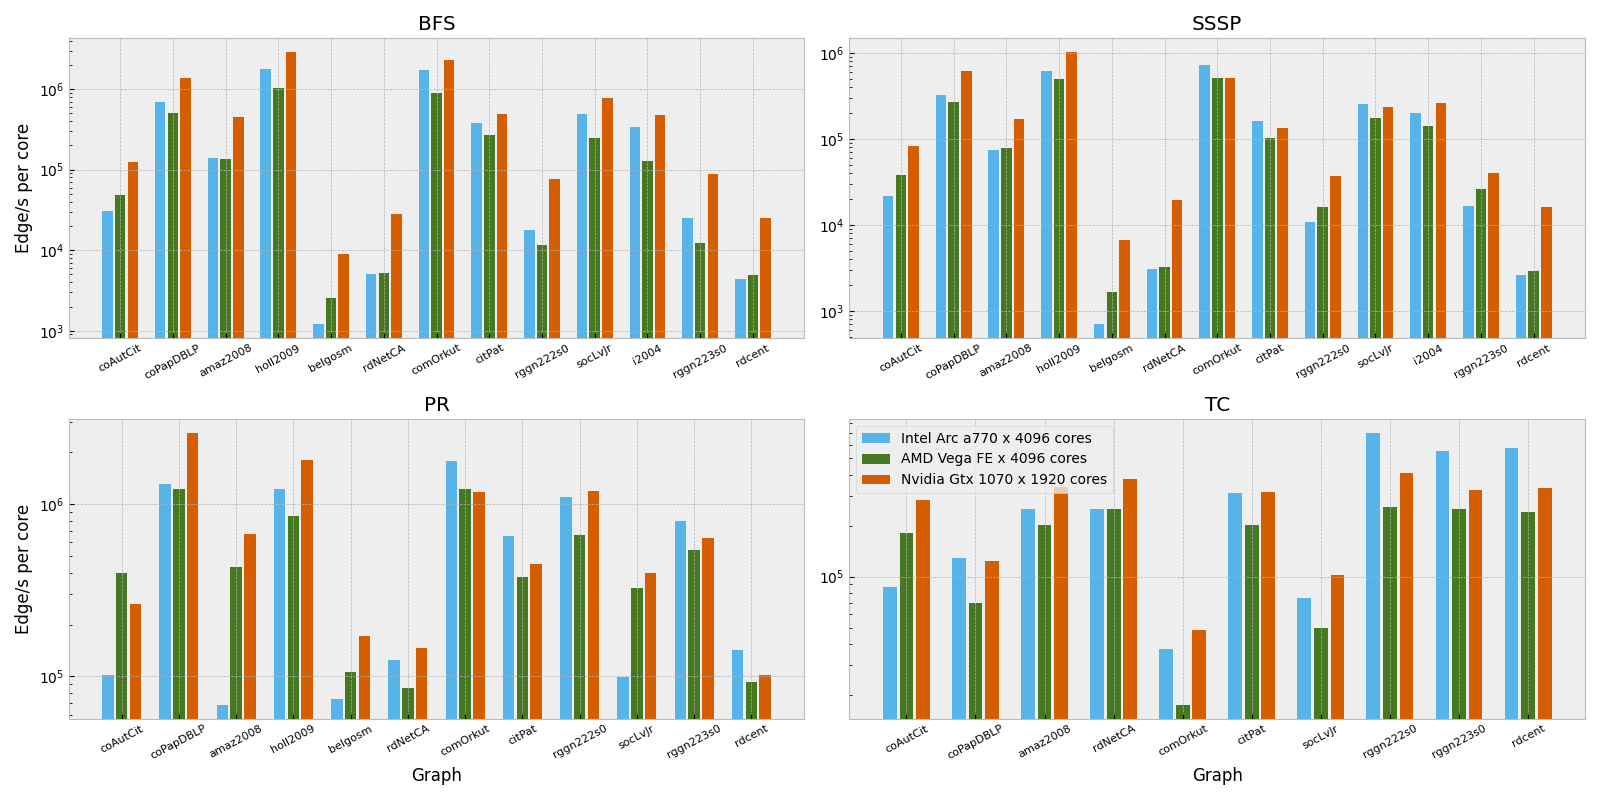
\includegraphics[width=0.85\linewidth]{pictures/rq2_cores.png}
    \\
    OpenCL, конечно, переносим, но всегда есть <<но>>
  \end{center}
\end{frame}

\begin{frame}
  \frametitle{Результаты на встроенной графике}
  \begin{center}
  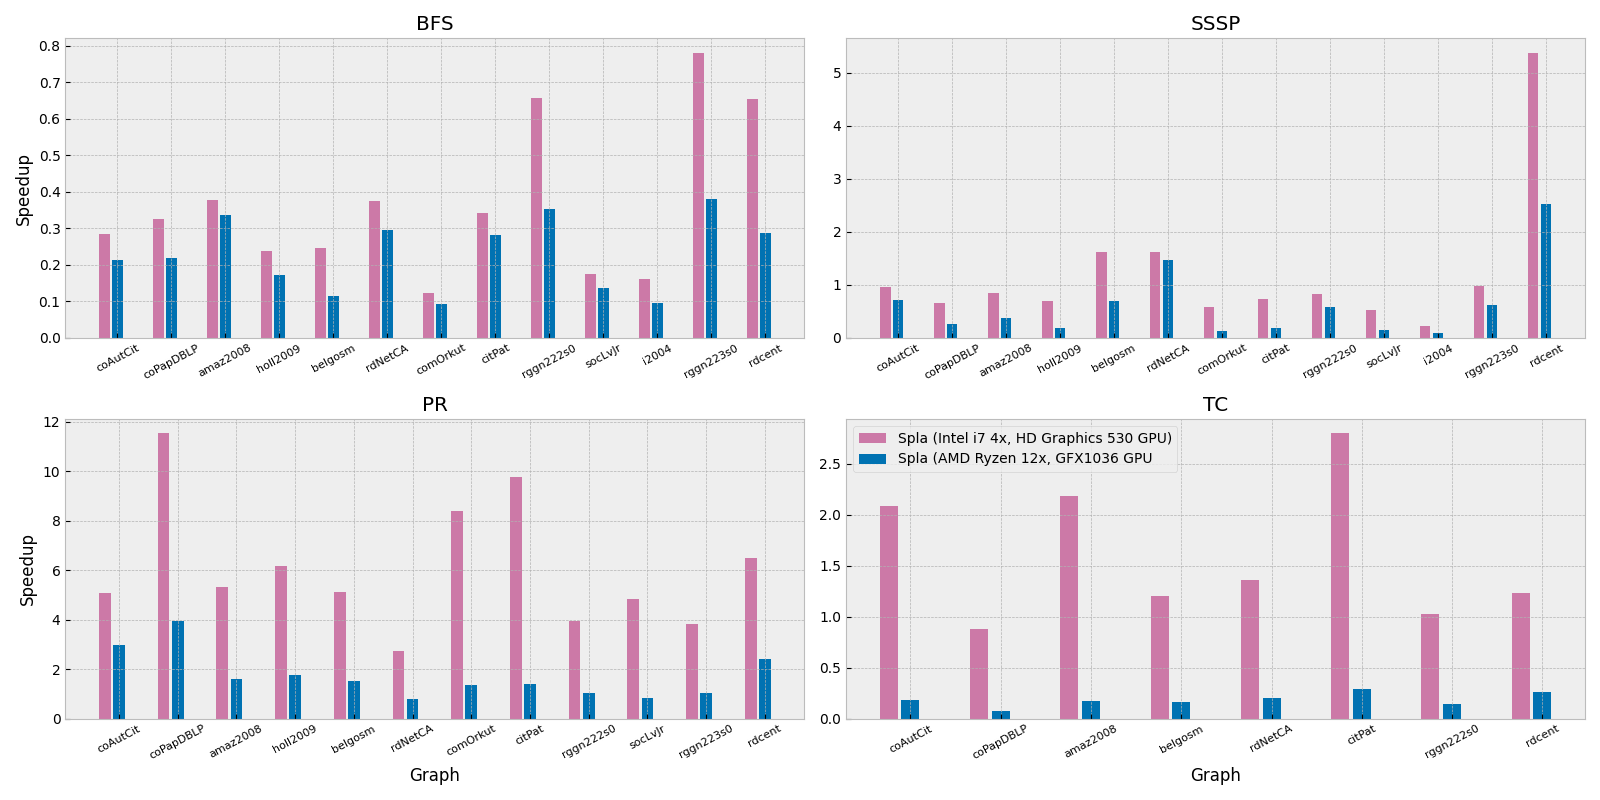
\includegraphics[width=0.85\linewidth]{pictures/rq3_int.png}
  \\
    Драйвер --- это важно!
  \end{center}
\end{frame}

\begin{frame}
  \frametitle{Результаты умножения матриц на GPGPU от Imagination Technologies}
  \begin{center}
  \tikzmark{z1}{ }
  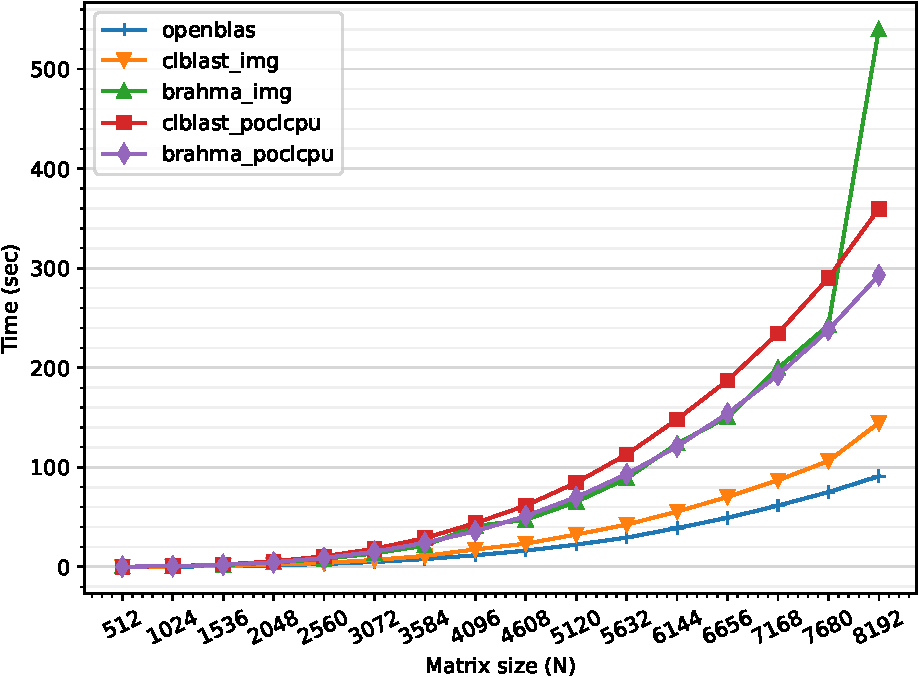
\includegraphics[width=0.55\textwidth]{pictures/MILK-V_crop.pdf}
  \tikz[overlay,remember picture]{\draw[draw=red,thick,double,fill opacity=0.2] ($ (z1) + (1.1,5.45)$) rectangle ($ (z1) + (3.4,6.05)$);}
  \\
    GPGPU от Imagination Technologies (пока) не совсем для вычислений
  \end{center}
\end{frame}

\begin{frame}[fragile]
  \frametitle{Пара слов про \href{https://github.com/vortexgpgpu/vortex}{Vortex}}
  \begin{itemize}
    \item Набор инструкций, основанный на RISC-V ISA
    \item Поддержка OpenCL через POCL 
    \begin{itemize}
      \item[\faGears] Spla должен запускаться
    \end{itemize}
    \item Проблемы со сбросом регистров
    \begin{itemize}
      \item Типичные оптимизации не работают
      \item \href{https://github.com/vortexgpgpu/vortex/issues/251}{Issue 1}
      \item \href{https://github.com/vortexgpgpu/vortex/issues/205}{Issue 2}
    \end{itemize}
    \item В целом, есть подозрение, что мало регистров
    \item Для ПЛИС с HBM
    \begin{itemize}
      \item[\faQuestion] Бонус для обработки слабоструктурированных данных
    \end{itemize}
  \end{itemize}
\end{frame}

\begin{frame}[fragile]
  \frametitle{Выводы}
  \begin{itemize}
    \item Обработка графов на GPGPU возможна и иногда полезна
    \begin{itemize}
      \item Для некоторых алгоритмов полезнее, чем для некоторых других
      \item Сильно зависит от структуры графа
    \end{itemize}
    \item OpenCL работает и для GPU и для CPU
    \begin{itemize}
      \item В том числе, для RISC-V      
    \end{itemize}
    \item Пока нет поддержки Cuda, выбор инструментов для обработки графов на GPU под RISC-V очень ограничен
    \begin{itemize}
      \item Фактически, только Spla
      \item В любом случае, OpenCL даёт хоть какую-то переносимость и независимость от вендора (и даже наличия GPU как такового)
    \end{itemize}
  \end{itemize}
\end{frame}
 
\begin{frame}[fragile]
  \frametitle{Возможные направления}
  \begin{itemize}
    \item Запуск Spla на Vortex
    \item Анализ производительности Spla на различных CPU и GPGPU    
    \item Оптимизация Spla
    \item Расширение возможностей Spla
    \item Запуск различных GPU (AMD, Intel) на платах с RISC-V
  \end{itemize}
\end{frame}


\end{document}
